
%Chapter 1

\renewcommand{\thechapter}{1}

\chapter{Introduction}


%We must proceed in life as kittens... into the box, out of the box, pause, into the box again, then out of the box just in time for more food...

A few centuries ago one of the greatest strides in astronomy was made by Kepler working off Tyco Brahe's data in understanding planetary orbits. Kepler discovered that planets move along elliptical orbits with the sun at one of the foci and thus developed the laws of planetary motion, along with the fact that it's useful to share data. In 1609 the concept was revolutionary yet it raised a more interesting question, why do planets move in elliptical orbits? Kepler explanation was that each planet was guided in its elliptical orbit by a resident angel, illustrated in figure \ref{fig:Kepler}.

\begin{figure}[h!]\centering
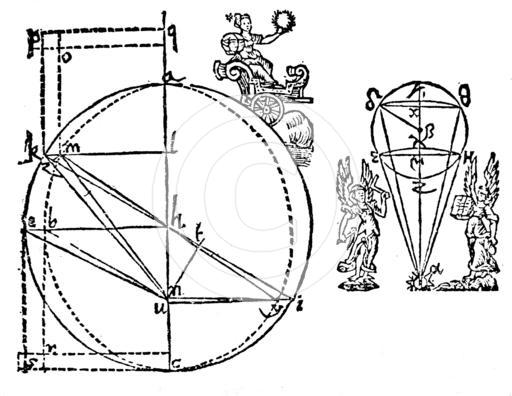
\includegraphics[width=120mm]{Intro/Ch1_Figures/Keplar.jpg}
\caption{Kepler explains the elliptical orbit of Mars, held fixed by a resident angel guiding its orbit.}
\label{fig:Kepler}
\end{figure}
 
Two hundred and fifty years later, another significant discovery was made on the nature of light by James Maxwell. Apparently, the light from mars shining into Tyco Brahe's eye (unaided by a telescope) had propagated through space as an electro magnetic wave. The propagation of light through a vacuum would require electric fields without the presence of charge, thus it was proposed that the universe is filled with aether through which electromagnetic waves could propagate. 

Fast forward to the era of the standard model, and  precision cosmology . The standard model provides as a nearly perfect framework to understand the interactions of particles we know of. Precision cosmological measurements are now constraining parameters deemed impossible several decades ago (Plank is a huge step up from Tyco's eye ball).  These measurements have provided the basis for the concordance cosmological model ($\rm \Lambda CDM$). Apart from knowing that planets move in elliptical orbits we also know that the universe is primarily composed of dark energy (69.2\%) and dark matter (25.8\%). Ordinary particles described by the standard model which compose our current understanding of `everything' only constitute 4.82\% of the universe. See figure \ref{fig:Lambda_CDM} for a diagram of the concordance cosmological model.

\begin{figure}[h!]\centering
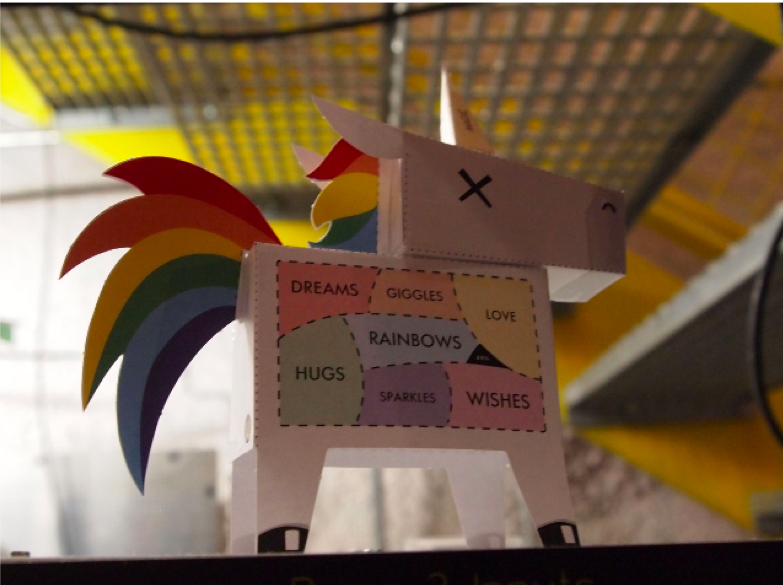
\includegraphics[width=150mm]{Intro/Ch1_Figures/Lambda_CDM.png}
\caption{$\rm \Lambda CDM$ parameters depicted on a unicorn by the LUX detector. The magic component which comprise the horn has yet to be directly detected, however it provides the backbone for the model. Note, the parameters in the diagram may not be representative of the specific universe in which this thesis is published.}
\label{fig:Lambda_CDM}
\end{figure}


%We have achieved a great strides measuring precisely that we are surrounded by five times more mass than the ordinary matter which we can see or feel. Raising the standard four year old questions, why?, where?, when?, what is it? The first we disregard as an impossibility to answer. The leading theories indicate that dark matter is gravitationally bound and distributed in a halo like structure around galaxies but we can't definitively answer that until we can detect it. When is now. A leading candidate for dark matter is a particle which carries mass and only couples gravitationally and hopefully couples the elctroweak force so that we can have a chance of ever directly observing it.  

%We proceed with exploring the box, after having feasted.... a century from now will seem like kittens trapped in a box, playing with xenon, leaving behind only a mass underground Unicorn art galleries in Lead SD?... we were here searching for dark matter, TS dump, bolt seized, ACRS forced xenon recovery, slow control computer crash, the DAQ is shooting lighting bolts (over a hundred unicorns drawing are posed in the underground control room ...and counting)

\section{Outline of Thesis}

In this section we review current cosmological evidence for the existence of dark matter, and give an overview of dark matter candidates along with the WIMP model. We also review if WIMPs existes how they could be detected and the and how scattering off a nuclei would look.

In Chap.\ 2, We overview the LUX detector, a liquid xenon time projection chamber (TPC), and how it searchers for WIMPs. We conclude the chapter with the most recent LUX science results which holds the worlds leading limit for spin independent WIMP nucleon scattering cross section.

In Chap.\ 3, the position dependent corrections of energy deposition in the LUX detector are discussed.

In Chap.\ 4, the absolute energy scale calibration of the LUX detector is discussed.

Chapter 5 ... (more to come) provides the conclusion to the thesis.

\section{Evidence for Dark Matter}

Astronomical observations hinting at the existence of dark matter were first observed in 1932 by Oort \cite{Oort} and more precisely in 1937 by Zwicky  \cite{Zwicky}. Both noted discrepancies in galactic mass measurements when comparing the luminous mass to the required to support galactic rotational velocities measured by red shifts. Oort had noted up to a factor of ten more mass than luminous mass in the Sombrero Galaxy and Zwicky found a factor of 500 for the Coma cluster. Both the observations were far to large to be accounted for by light absorption, indicating the existence of dark matter to account for the missing mass. Since then more evidence for the existence of dark matter has been compiled, including big bang nucleosynthesis (BBN), anisotropies in the cosmic microwave background (CMB), baryonic acoustic oscillations (BAO), formation of large structures, galactic ration curves, and gravitational lensing. All independent techniques leading to a unified conclusion for the existence of non baryonic and non luminous matter. Individually some pieces of evidence, such as galactic rotation curves, can be explained by modifications to general relativity (GR), but not all simultaneously. The existence of non relativistic, dark matter particles are required in order to unify the current observations. This dark matter does not couple to the electromagnetic force and is thus able to avoid our standard detection techniques, making its presence felt on large scales via gravity. In the last thirty years significant progress has been made in the direct detection of such a particle, the forefront of which will be presented in this thesis.

\subsection{Galactic Rotation Curves}

There are two common methods for measuring the mass of a galaxy or cluster of galaxies. First, one can use the total luminosity and the known distance to the galaxy to determine the luminous mass, that is the mass corresponding to the visible light. Second, the rotational velocities of stars orbiting the galactic center can be mapped and used to determine the mass distribution as a function of galactic radius. Rotational velocities of stars around galactic centers at large distances can be measured with Doppler shift, with more recent measurement relying on the 21 cm H1 line from hydrogen as the standard candle. The rotational velocities of objects orbiting galaxies are highly non relativistic moving at speeds on the order 100 km/s. At the outer edges of the luminous galactic centers, typically past 5 kpc the velocity distribution is expected to fall off as redacted by Newtonian mechanics $\sim$1/r. Yet observations from as early as 1932 indicate that velocity distributions tend to remain constant with radius suggesting that the objects are not rotating around the central luminous mass, rather they are rotating inside a solid body of dark matter \cite{Oort} \cite{Zwicky} \cite{Galactic_Velocities} \cite{DarkMatter_MW}. The velocity distributions measured for the Milky Way galaxy are show in \ref{fig:MW_Rotation}.

\begin{figure}[h!]\centering
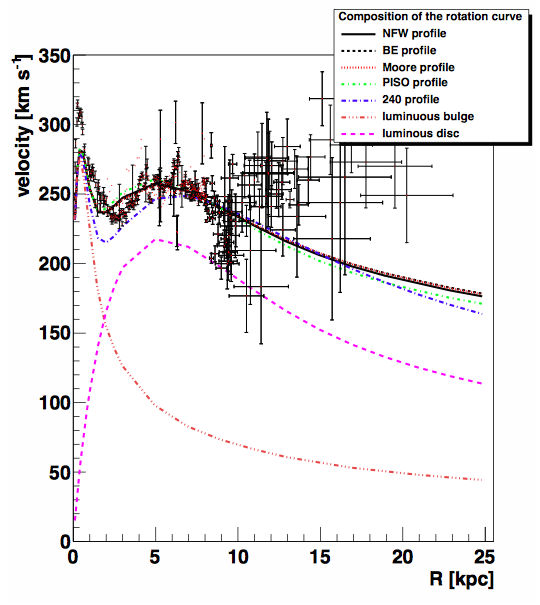
\includegraphics[width=120mm]{Intro/Ch1_Figures/MW_Rotation.png}
\caption{Measured rotational velocities vs. radius in the Milky Way galaxy. The velocity distribution is consistent with a halo of mass surrounding the galaxy well beyond the observed luminous disk \cite{DarkMatter_MW}. }
\label{fig:MW_Rotation}
\end{figure}

\subsection{BBN}

Big band nucleosynthesis (BBN) accounts for the relative abundances of light elements in the universe today, including H, D, $\rm He^3$, $\rm He^4$ and $\rm Li^7$ \cite{BBN}. BBN took place in a relatively short time window several seconds after the big bang when the universe cooled below $\rm10^{11}$K (10 MeV) and seized as the temperature cooled below $\rm10^9$K (100 keV). Under the temperature conditions of BBN it was energetically favorable for free protons and neutrons to undergo nuclear fusion and is the only mechanism to produce light elements we see today. The heavier elements were later fused together in stars and ejected upon the star's death into the cosmos. Nuclear cross sections of protons, neutrons and light elements have been measured to high person and can be combined with the expansion rate of the universe to precisely predict the relic abundances of baryonic matter. Observations constrain the abundances of the light elements to be H$\sim$ 75\%, D$\sim$ 25\%, $\rm He^4$ $\sim$ 0.01\%, $\rm Li^7$ $\sim 10^{-10}$ \%. The ratio of D/H has been used to constrain the relic density of baryonic matter to be $\Omega_b h^2$= 0.02202 $\pm$ 0.00046 \cite{OmegaB_BBN}.

\begin{equation}
\centering
\Omega_b h^2= \frac{p_b}{p_c}
\end{equation}

\noindent Where h is the Hubble constant H dividend by 100 ($\rm H_0/100$), $p_b$ is the baryonic density and $p_c$ is the critical density required for a flat universe (verified by the CMB). We can write the $\rm i^{th}$ density component as: 

\begin{equation}
\centering
\Omega_i \equiv \frac{p_b}{p_c} = \frac{8\pi G \rho_i}{3H^2}
\end{equation}

\noindent Where G is the gravitational constant, H is the Hubble constant (found in table \ref{table:Cosmo_Param}). The baryon density measured using BBN is constrained to within 1\% and in agreement with the latest constraints from Plank's CMB data, $\Omega_b h^2$= 0.02205 $\pm$ 0.00028 \cite{Planck_Param}.

\subsection{CMB}
\label{sec:CMB}
The early universe consisted of a plasma making the universe opaque to photons as they scattered off free electrons. As the temperature fell below the binding energy of hydrogen 13.6 eV, electrons neutral atoms allowing photons to decouple from the plasma making the universe became transparent. The mean temperature of decoupling was actually at 0.25 eV ($\sim$4000 K) as photons still scatter frequently near the binding energy of hydrogen \cite{BBN}. The cosmic microwave background (CMB) emanated from this time after making a final scatter photons decoupled from electrons effectively attaining a mean free path on the scale of the universe. The photons from the CMB observed today at the red shift temperature of 2.72548$\pm$0.00057 K \cite{CMB_Temp} have not interacted from the time of last scatter 379,000 years after the bing bang. The CMB has encoded within it a wealth of information about the universe as it was at the time of decoupling. The concept of the information encoding is illustrated in figure using Maru the cat in various boxes. Consider that Maru is a photon and the box size represents local energy densities of the universe. The smaller boxes represent areas of higher energy density and temperature. At the time of last scatter all boxes containing Marus cease to exist, to the horror of of the cats. The cats now begging to propagate freely through the universe with their configuration unchanged (the cats are too lazy to move and are content napping while propagating though space). It should be noted, that as the universe expands so will the cats. When the Marus finally reach our telescopes, 13 billion years latter,  the shape and squeezing of each Maru informs us of the box size (temperature) from which each Maru has emanated. Using this information from multiple Marus the distribution of box sizes at the time of last scatter can be mapped, reveling areas of slightly larger boxes and areas of slightly smaller boxes. This is roughly the idea behind measuring anisotropies in the cosmic microwave background using microwave telescopes. 

\begin{figure}[h!]\centering
 
\subcaptionbox{\label{fig:1a}}{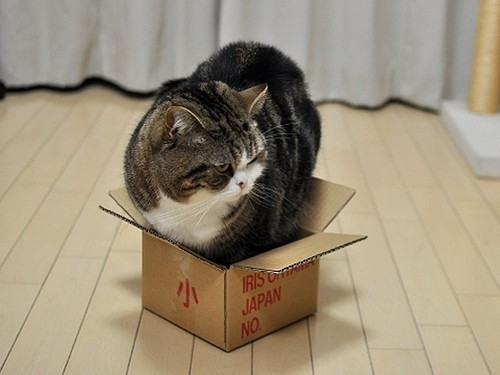
\includegraphics[width=72mm]{Intro/Maru/tiny_box.jpg}}
\hfill
\subcaptionbox{\label{fig:1b}}{
\includegraphics[width=72mm]{Intro/Maru/small_box_2.jpg}}


\bigskip

\subcaptionbox{\label{fig:1c}}{
\includegraphics[width=72mm]{Intro/Maru/medium_box_2.jpg}}
\hfill
\subcaptionbox{\label{fig:1d}}{
\includegraphics[width=72mm]{Intro/Maru/large_box.jpg}}

\caption{Maru the cat explains the cosmic microwave background. Consider that Maru is a photon and the box size represents local energy densities of the universe. The scale of the the box size is inversely proportional to the local energy density and temperature. At the time of last scatter all boxes containing Marus cease to exist, to the horror of of the cats! The Marus are now left to propagate freely through the universe, with their configurations unchanged (the cats are too lazy to move and are content napping for 13.7 billion years). Figures a-d show Maru the cat contained within increasing box sizes corresponding to decreasing energy densities.}
\label{fig:CMB_Maru}
\end{figure}



 .Ever more increasing measurements from COBE, WMAP and Planck have been able to probe slight temperature variations to 1 part in 100,000 as seen in figure \ref{fig:CMB_Hist}. Table \ref{table:Cosmo_Param} shows the constraints on cosmological parameters set by Planck. The results are in good agreement with baryonic density derived from BBN and predict a dark matter component of 25.8\%.

\begin{figure}[h!]\centering
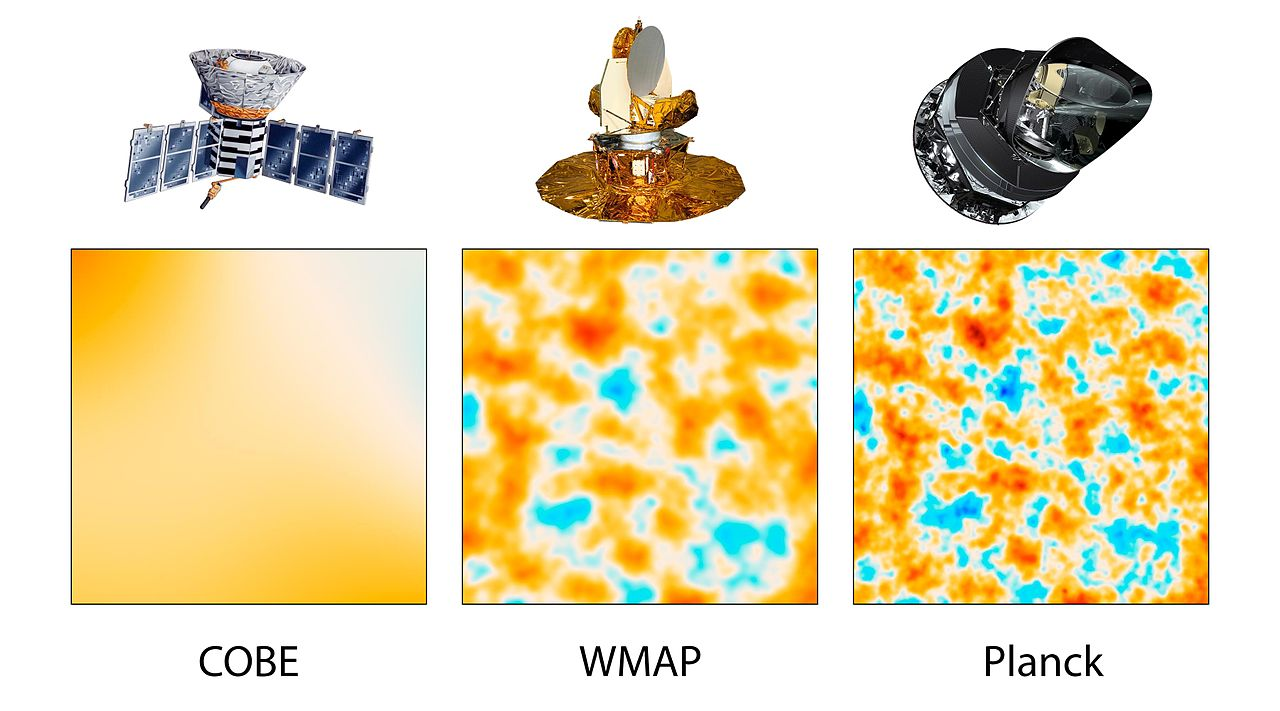
\includegraphics[width=130mm]{Intro/Ch1_Figures/CMB_Hist.jpg}
\caption{Improvement of resolution from COBE, first to discover anisotropies in the CMB, to WMAP and Planck which have set stringent limits on cosmological parameters by mapping variations in temperature of 1 part in 100,000. Image credit: NASA/JPL-Caltech/ESA. }
\label{fig:CMB_Hist}
\end{figure}

\renewcommand{\baselinestretch}{1}
\small\normalsize

\begin{table}[h!]
%\footnotesize
\begin{center}
\begin{tabular}{|c|c|c|c|c|c|}
\hline
Parameter & Value & Definition\\ \hline
$\Omega_bh^2 $ 		& 0.2214$\pm$0.00024 		&Baryon energy density \\ \hline
$\Omega_ch^2 $ 		& 0.1187$\pm$0.0017			& Cold dark matter energy density\\ \hline
$\Omega_mh^2 $ 		& 0.1423$\pm$0.0029 $^*$ 	& Total matter energy density\\ \hline
$\Omega_{\Lambda}$& 0.692 $\pm$ 0.010			&  Dark energy density \\ \hline
$\Omega_K$ 			& -0.0005$\pm$0.0065 (95\%) & Curvature\\ \hline
$\Sigma_{m_v}$		& $<$ 0.230 					& Sum of neutrino masses [eV] \\ \hline
$H_0$ 					& 67.77$\pm$0.77				& Hubble Constant [$\rm km s^{-1} Mpc^{-1}$]\\ \hline
\end{tabular}
\caption{Cosmological parameters from Planck+WP+highL+BAO \cite{Planck_Param}. $^*$ Only Planck.}
\label{table:Cosmo_Param}
\end{center}
\end{table}

\renewcommand{\baselinestretch}{2}
\small\normalsize

\subsection{BAO}

The universe 379,000 years after the big bang was uniformly distributed, with only small variations observed in the CMB temperature of 1/100,000 \cite{Plank_Map}. Before decoupling took place gravity pulled baryons and dark matter into high density regions resulting in an opposing outward force from photon pressure. The outward force from the photon pressure was only felt by the baryons whereas the dark matter component would not not couple to photons. The competing attractive and repulsive forces gave rise to baryonic acoustic oscillations (BAO) with density regions propagating as spherical sound waves do. The amplitudes of the waves are separated by a characteristic radius called the sound horizon r, which is sensitive to the initial dark matter and baryon densities \cite{BAO_Theory}. Anisotropies in the CMB power spectrum probe these oscillations as discussed previously in \ref{sec:CMB}. At the time of decoupling the photon pressure ceased providing the opposing force allowing the gravitational restoring force to dampen the oscillations. If the picture since the time of the CMB is propagated forward in time we expect that areas of the CMB that were denser would cluster, thus statistically the universe is expected to have large scale structures on the order of the sound horizon r. Measurements of BAO by the Sloan Digital Sky Survey \cite{Sloan} and BOSS \cite{BOSS}are consistent with the sound horizon expected from anisotropies in the CMB, with a preferred scale of $\rm 100hh^{-1}$ Mpc ($\sim$150 Mpc) between large scale structures. Figure {fig:BOSS} shows the result from BOSS using Lyman-$\alpha$ absorption in quasar emission spectrum due to the presence of neutral hydrogen in the intergalactic medium \cite{BOSS}.

\begin{figure}[h!]\centering
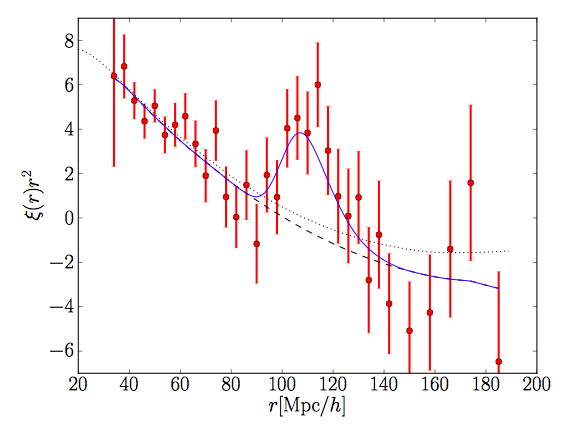
\includegraphics[width=120mm]{Intro/Ch1_Figures/BOSS.png}
\caption{BAO peak obtained from BOSS \cite{BOSS} }
\label{fig:BOSS}
\end{figure}

\subsection{Gravitational Lensing}

Gravitational lensing can be to map the focal points of gravitational mass in a galaxy or cluster. The idea is to look for repeating structures around a large central mass which have been bent around regions of large mass. These repeating structures are caused by light trajectories bending before reaching earth creating an optical illusion, appearing as if the light had emanated from multiple sources along a straight lines of sight. Observations of the Bullet cluster strongly support the existence of dark-matter. The Bullet cluster is made up of two galaxy clusters which have recently collided and passed through each other. The collision has caused the ordinary, baryonic matter to heat and emit X-rays that are observed and used to map the luminous mass distribution \cite{Bullet_Cluster_Xray}. However, the observed concentration of mass is not consistent with the center of mass observed using gravitational lensing via GR \cite{Bullet_Cluster_DM}. The way light bends around the bullet-cluster would indicate the presence of a dark-matter shell which, unlike the ordinary matter, has passed through at a faster rate due to the lack of interactions. Figure \ref{fig:Bullet} shows the concentration of mass in the bullet-cluster as observed from X-rays, emitted by baryonic matter, in pink and the concentration of mass from gravitational lensing in blue. The X-ray mapping from Chandra when compared with  gravitational lensing studies of the Bullet cluster clearly demonstrate a decoupling of the dark matter center of mass from the baryonic center of mass induced by the cluster's recent collision.

\begin{figure}[h!]\centering
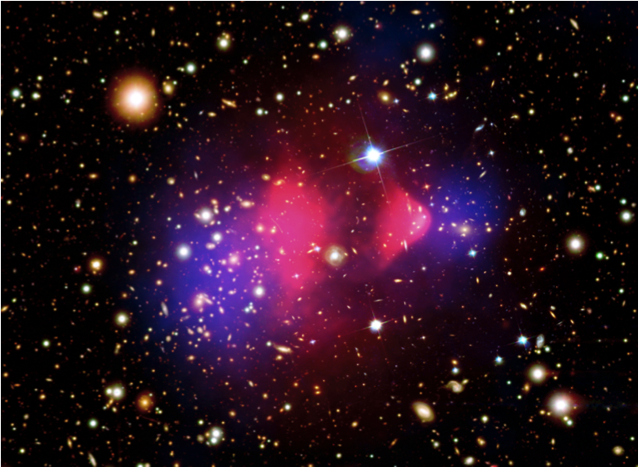
\includegraphics[width=130mm]{Intro/Ch1_Figures/Bullet_Cluster.png}
\caption{The concentration of mass in the bullet-cluster as observed from X-rays, emitted by baryonic matter, in pink and the concentration of mass from gravitational lensing in blue. [Composite image credit: X-ray: NASA/CXC/CfA/M.Markevitch et al.; Optical: NASA/STScI; Magellan/U.Arizona/D.Clowe et al.; Lensing Map: NASA/STScI; ESO WFI; Magellan/U.Arizona/D.Clowe et al.] }
\label{fig:Bullet}
\end{figure}


%\subsection{$\rm \Lambda CDM$}

\section{Dark Matter Candidates}

The evidence for the existence of missing mass outlined in the previous section forces us to examine solutions to account for those cosmological phenomina. It is natural to at first try and solve the anomaly by using our understanding of standard model particles. The first candidate considered for dark matter is the existence of Massive Compact Halo Objects (MACHOs). However, the MACHO theory requires that the extra mass be baryonic which is refuted by the precision measurements (BBN, CMB) that limit Baryonic mass to only 2.2\% while the overall matter energy density required is 31.75\% \cite{BBN_Constraints} \cite{Planck_Param} (see table \ref{table:Cosmo_Param}).
A non baryonic candidate drawn from the standard model are neutrinos, which are known to carry mass due to oscillations and only interact weakly \cite{SNO}. However, large scale structure formation require that the universe have a `cold' ( non relativistic)dark matter component in order to become gravitationally bound to galaxies. With current constraints on the neutrinos masses to less than 0.23 eV \cite{Planck_Param}, neutrinos are highly relativistic and would fail to reproduce structuring of the universe observed today \cite{Neutrino_DM}.

\subsection{AXIONS}
\begin{footnotesize}``I named them after a laundry detergent, since they clean up a problem with an axial current" � Frank Wilczek
\end{footnotesize}


Axions were introduced to solve the strong CP problem. The Lagrangian allowed by gauge symmetry includes a term
\begin{equation}
\centering
\rm \mathcal{L}=\Theta \frac{g_s^2}{32\pi^2}G^{a}_{\mu \nu}\widetilde{G}^{\mu \nu a}
\end{equation}

\noindent where g is the gluon QCD coupling constant, $\rm G^{a}_{\mu \nu}$ the gluon field strength and $\rm \Theta$ is a constant \cite{AXION_Theory}. The Lagrangian breaks gauge symmetry which allows for CP violating and is expected to contribute to the electric dipole moment (NEDM). Measurements of the NEDM have been constrained to be much smaller than expected with CP violation. NEDM is constrained to be less than $\rm 2.9\times10^{-26}$ e cm (90\% CL) \cite{NEDM}, resulting in $\rm \Theta$ of less than $\rm 0.7 \times 10^{-11}$.

An elegant solution for the lack of observe red electric dipole moment was introduced by Pecci and Quinn. The proposed idea is to promote $\rm \Theta$ to a dynamical field value through a new symmetry (PQ symmetry) which is spontaneously broken naturally leading to $\rm \Theta=0$ by minimizing the potential  \cite{PQ1} \cite{PQ2}. Such a solution to the strong CP problem leads to the existence of a light pseudo scalar particle, the Axion. The axion would be a light particle which could couple to the electromagnetic field, in the presence of a strong electromagnetic field, $ \rm \textit{a} \leftrightarrow \gamma \gamma $ \cite{CAST}.

\begin{figure}[h!]\centering
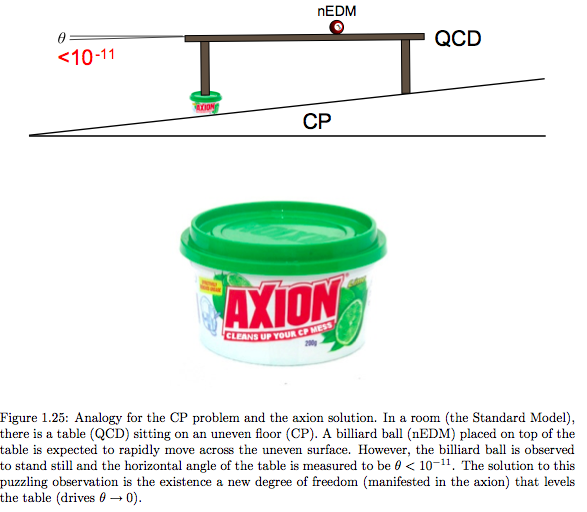
\includegraphics[width=120mm]{Intro/Ch1_Figures/Carlos_Axions.png}
\caption{Illustration of the CP problem and the axion solution. ``Analogy for the CP problem and the axion solution. In a room (the Standard Model), there is a table (QCD) sitting on an uneven floor (CP). A billiard ball (nEDM) placed on top of the table is expected to rapidly move across the uneven surface. However, the billiard ball is observed to stand still and the horizontal angle of the table is measured to be $\theta < 10^{-11}$. The solution to this puzzling observation is the existence a new degree of freedom (manifested in the axion) that levels the table (drives $\theta$ 0)", [Carlos' Thesis] }
\label{fig:Carlos_Axions}
\end{figure}


Searches for axions involve looking for the rare electromagnetic interactions that convert axions into microwaves in resonating cavities with large magnetic fields here on earth. ADMX has been sensitive to mass scales of 3.3 $\rm \mu eV$ to 3.59 $\rm \mu eV$ with planned upgrades to explore more parameter space \cite{ADMX}. Coupling of photons to axions could also occur in the strong electromagnetic fields of our own sun. The CAST experiment searches for axions produced in the interior of the sun from thermal photons, with keV energies, which then arrive to the detector where they are converted back into X-rays within a large dipole magnet \cite{CAST}. The axion solves the strong CP problem and is a potential dark matter candidate, there is still vast parameter space to explore with potential axion massed ranging from $\rm \mu eV$ to eV scales. Instruments are being upgraded to explore these regions and will require patience, since each potential axion mass requires tuning the cavity to a specific resonance and waiting.

\subsection{WIMPs}

A leading candidate to explain the dark matter is weakly interacting massive particle (WIMP), as the name implies is a massive that only couples via the weak interaction and also gravity. The WIMP is theorized to have a mass and cross section on the order of the weak interaction. In the early universe the number density of WIMPs and photons would have been roughly equation as there was sufficient thermal energy keep the creation and annihilation in equilibrium. 
\begin{equation}
\chi \chi \rightleftharpoons qq
\end{equation}
\noindent $\chi$ represents WIMPs and q are standard model particles. The reaction can go back and forth in equilibrium as long as the thermal temperature of the universe is greater than WIMP mass $\rm T>m_\chi$.

As the universe expanded and cooled production of WIMPs from standard model particles cease as the temperature of the universe dropped below the WIMP mass, leaving only WIMP annihilation into standard model particles. The annihilation process of WIMPs would have continued leaving only a small number density at the tail of an exponentially falling Boltzmann distribution today. However, if the universe's expansion is fast compared to the WIMP cross section then the WIMPs would have avoided finding each other and their number density could `freeze out'. Thus, if the acceleration of the universe H is greater than the number density of WIMPs times the cross section.
\begin{equation}
\rm H>\Gamma_A\equiv n_\chi \left<\sigma_A \nu \right>
\end{equation}
\noindent H is the Hubble constant , $\rm n_\chi$ is the number density of WIMPs and $\rm \left<\sigma_A \nu \right> $ is the thermally averaged annihilation cross-section. The annihilation process can be described by the Boltzmann equation
\begin{equation}
\rm \frac{dn}{dt}=-3Hn_\chi -\left<\sigma_A \nu \right>(n_\chi^2-n_{\chi_{eq}}^2)
\label{eq:Freeze}
\end{equation}

\noindent Where the first term represents the dilutions of WIMP number density with three degrees of freedom. $n_\chi^2$ is from the annihilation process, $\chi\chi \rightarrow qq$ and $n_{\chi_{eq}}^2$ is from the reverse process $qq \rightarrow \chi\chi$. Equation \ref{eq:Freeze} does not have an analytic solution but has been solved numerically\cite{WIMP_Freeze} , estimating the relic density within 10\% to be:
\begin{equation}
\Omega_\chi h^2 = \frac{3\times10^{-27} \mathrm{cm^3 s^{-1}} }{\left<\sigma_A \nu \right>} \sim \frac{10 ^{-10} \mathrm{GeV}^{-2} }{\left<\sigma_A \nu \right>}
\label{eq:WIMP_Relic}
\end{equation}

\noindent Using a typical weak scale cross-section in equation \ref{eq:WIMP_Relic},
\begin{equation}
\left<\sigma_A \nu \right> \sim \frac{\alpha^2}{m_{weak}^2} \sim 10^{-9} \mathrm{GeV}^{-2}
\end{equation}

\noindent We find that the relic WIMP density reduces to $\Omega_\chi h^2$ = 0.1 for a particle with a weak scale interaction, referred to as the WIMP miracle. In good agreement with the expected cold dark matter component of the universe $\Omega_{c}h^2 = 0.12029  \cite{Planck_Param}$


\section{WIMP Dark Matter Searches}

There are three methods for detecting WIMPs other than looking for its gravitational effects. First, we can look for the annihilation of dark matter particles into standard model particles using space telescope based experiments. Second, we could try to produce dark matter particles by colliding standard model particles in accelerators  and look for a signature of missing energy. Or we can search for rare collisions of dark matter particles with ordinary matter. The first two options would constitute indirect observations as only a standard model particle or missing energy is detected to infer the existence of dark matter, this introduces significant systematics and potential fake signals. The third option is rather attractive as it involves directly observing a collision with a dark matter particle though it too come along with significant challenges, mainly it requires a near zero background environment in order to observe the additional flux.

\begin{figure}[h!]\centering
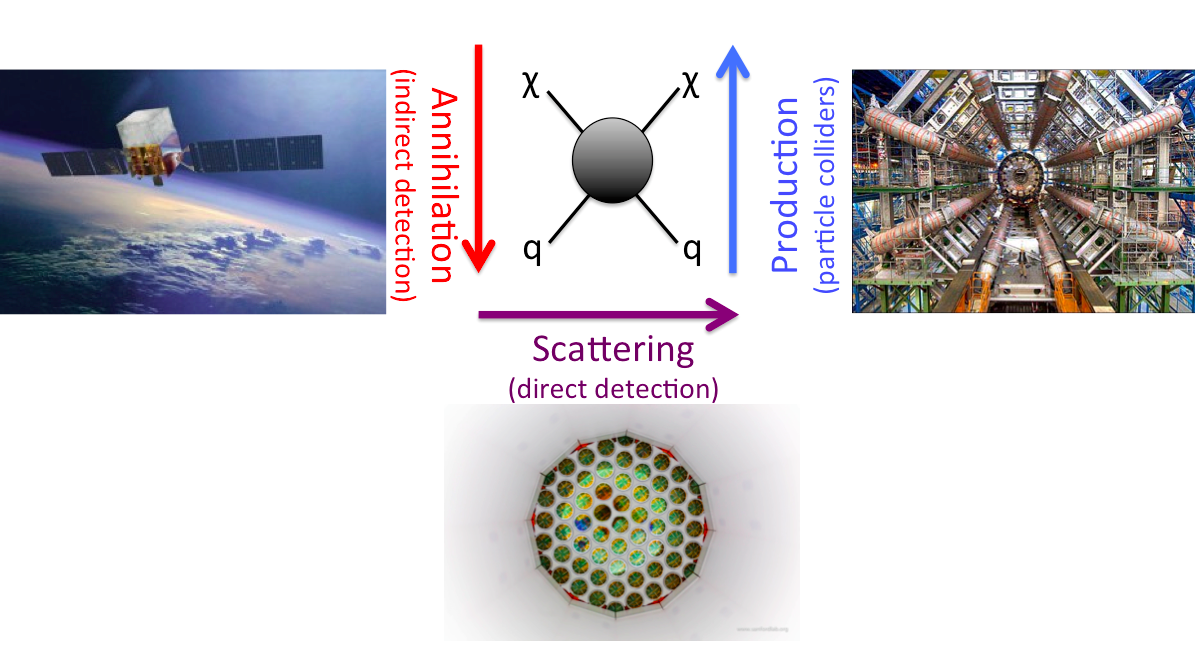
\includegraphics[width=130mm]{Intro/Ch1_Figures/DM_Detection.png}
\caption{Methods for detecting WIMPs from interactions of q, standard model particles, and dark matter particles $\chi$. WIMPs can be detected through the annihilation of dark matter particles into standard model particles, $\rm \chi\chi \rightarrow qq$. WIMPs can be produced by colliding standard model particles, $\rm qq \rightarrow \chi\chi$. Or one can look for the scatter of a dark matter particle off a standard model particle, $\rm \chi q \rightarrow \chi q$. }
\label{fig:DM_Detection}
\end{figure}

\newpage

\subsection{Direct Detection}

WIMPS could have masses in the GeV to TeV range and would comprise a quarter of the total mass of the universe. The local density of WIMPs around the earth, at 8 kpc from the galactic center, is about 0.3 GeV/$\rm cm^3$, estimated from the galactic rotation curve of the Milky-Way with the assumption of a halo like distribution (figure \ref{fig:Local_DM} and \cite{DarkMatter_MW}). Assuming that the WIMP mass is on the order of the weak scale, 100GeV, there are roughly three proton masses worth of WIMPs per liter of space. The velocity of WIMPs near the Earth is about the orbital velocity of objects about the galactic center 240km/s at 8.3 kpc, shown in figure \ref{fig:MW_Rotation}. WIMPs being highly non-relativistic would scatter coherently off of target nuclei with a cross-section corresponding to $\rm \sim A^2$. 

\begin{figure}[h!]\centering
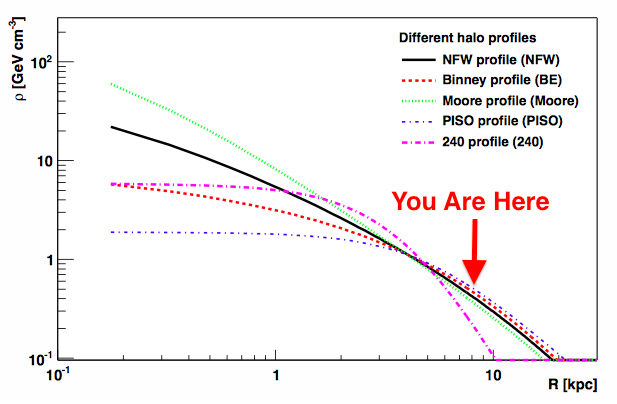
\includegraphics[width=130mm]{Intro/Ch1_Figures/DM_Dist_MW.png}
\caption{Dark matter density vs. distance from the galactic center, calculated from galactic rotation curves of the Milky Way galaxy. The Earth is located at 8.3 kpc. Figure from \cite{DarkMatter_MW}.  }
\label{fig:Local_DM}
\end{figure}


WIMP scattering off of target nuclei can be expressed as a classical inelastic collision. The most common energy deposit can be expressed as

\begin{equation}
\rm E_{max}=r\cdot E_0 = \frac{r}{2}M_\chi v^2
\end{equation}

\noindent Where $\rm E_{max}$ is the most frequent energy deposit, $\rm M_\chi$ is the WIMP mass and v is the WIMP velocity. The kinematic factor r for isotropic scattering off a target mass $\rm M_T$ in the laboratory frame is given by (using 1/2 as the average of 1-cos$\rm \theta$.):
 
\begin{equation}
\rm r= \frac{4M_\chi M_T}{(M_\chi +M_T)^2}
\end{equation}

\noindent Assuming classic billiard ball scattering we calculate expected energy deposits for various WIMPs with weak scale masses of 1 to 1000 $\rm GeV/c^2$. Using xenon as the target mass ($\rm M_{Xe}=122 \, GeV/c^2$), and a WIMP velocity of 240 km/s ($\rm 8\times 10^{-4}$ c ).

\renewcommand{\baselinestretch}{1}
\small\normalsize

\begin{table}[h!]
\begin{center}
\begin{tabular}{|c|c|c|}
\hline
$\rm M_\chi$ [$\rm GeV/c^2$] 	&	r 		&	$\rm E_{max}$ [keV] \\ \hline
1									& 0.032	& 0.01 \\ \hline
10									& 0.28		& 0.90 \\ \hline
100								& 0.99		& 31.7 \\ \hline
10000								& 0.40		& 124 \\ \hline
\end{tabular}
\end{center}
\caption{The kinematic factor r and most common energy deposit $\rm E_{max}$ for a WIMP of mass $\rm M_\chi$ scattering off a xenon nucleus.}
\label{table:WIMP_Deposit}
\end{table}

\renewcommand{\baselinestretch}{2}
\small\normalsize

To calculate the WIMP-target scattering event rate we follow the derivation given by Lewin and Smith \cite{Lewin_Smith}. The differential rate of the WIMP nuclear recoils will be an exponentially decaying spectrum.

\begin{equation}
\rm \frac{dR}{dE_R}=\frac{R_0}{E_0r}e^{-E_R/E_0r}
\label{eq:WIMP_Rate_1}
\end{equation}

\noindent $\rm E_R$ is the recoil energy, $\rm E_0$ is the most probable WIMP kinetic energy, r is the kinematic factor, R is the event rate per unit mass and $\rm R_0$ is the total rate. The event rate dR scattering off a tater size A can be written as

\begin{equation}
\rm dR=\frac{\mathcal{N}_0}{A}\sigma \nu dn
\label{eq:dR}
\end{equation}

\noindent Where $\rm \mathcal{N}_0$ is Avagadro's number, A is the atomic mass, $\rm \sigma$ is the atomic mass, $\rm \nu$ is the WIMP velocity and dn is the differential number density of WIMPs given by:

\begin{equation}
\rm dn=\frac{n_o}{k}\mathcal{F}(\nu, \nu_E)d^3\nu
\label{eq:dn}
\end{equation}

\noindent Where k = $\rm (\pi \nu_0^2)^{3/2}$ as $\nu_{esc} \rightarrow \infty$, an approximation good to within 0.5\% for the Milky Way.  $\rm n_o$ is the particle number density ($\rm n_o = p_\chi / m_\chi$). The WIMP velocity distribution $\rm \mathcal{F}(\nu, \nu_E)$ is assumed to be ideal gas described by a Maxwellian distribution:

\begin{equation}
\rm \mathcal{F}(\nu, \nu_E) = e^{-(\nu+\nu_E)^2/\nu_0^2}
\end{equation}

\noindent Where $\rm \nu$ is the WIMP velocity, $\rm \nu_E$ is the earth velocity, $\rm \nu_0$ is the average velocity (about 230 km/s). We now rewrite equation \ref{eq:WIMP_Rate_1} interns of an integral over all possible velocities rather than energy and plug in the result for dR (\ref{eq:dR}) and dn (\ref{eq:dn}) leading to :

\begin{equation}
\rm \frac{dR}{dE_R}=\frac{R_0}{E_0r}\frac{1}{k}\frac{1}{2\pi \nu_0^2}\mathlarger{\int}\limits_{\mathsmaller \nu_{min}}^{\mathsmaller \nu_{max}} \frac{1}{\nu}\mathcal{F}(\nu, \nu_E)d^3\nu
\end{equation}

\noindent $\rm R_0$ absorbs the constants $\rm R_0 = \frac{2}{\pi^{1/2}}\frac{\mathcal{N_0}}{A}\frac{\rho_\chi}{M_\chi}\sigma_T\nu_o $.

Having solved for the differential rate we now calculate the spin independent cross section for WIMPs scattering off nucleons of an atom ($\rm \sigma_T$). We write the cross section as a sum off scattering off protons and neutrons in the nucleus. We use the fact that nucleon coupling for protons and neutrons is approximately equal \cite{Fp_Fn}.

\begin{equation}
\rm \sigma_T = \frac{4\mu^2A}{\pi} [Z\cdot \mathit{f_p} + (A-Z) \mathit{f_n} ] \approx \frac{4 \mu^2 A^2}{\pi} \sigma_n
\end{equation}

\noindent Where $\rm \mu$ is the reduced mass of the WIMP  nucleon system given by:

\begin{equation}
\mu=\frac{M_\chi M_n}{M_\chi + M_n}
\end{equation}

\noindent Finally we must add the specific nuclear form factor for the specific target atom to account for decoherence, described by the Helm factor \cite{Helm_Factor} F(q). The cross section for spin independent scattering off the target nucleus can be written as a product of the idealized cross section and Helm factor:

\begin{equation}
\rm \sigma_T(q)= \sigma_TF^2(q)=\frac{4A^2}{\pi}\left(\frac{M_\chi M_n}{M_\chi + M_n}\right)^2\sigma_nF^2(q)
\end{equation}

The spin-independent cross section for WIMPs is found to be proportional to the atomic number squared ($\rm A^2$). The event rate per nuclear recoil energy is plotted for several potential WIMP search target nuclei in figure \ref{fig:WIMP_Target_Nuclei}.

\begin{figure}[h!]\centering
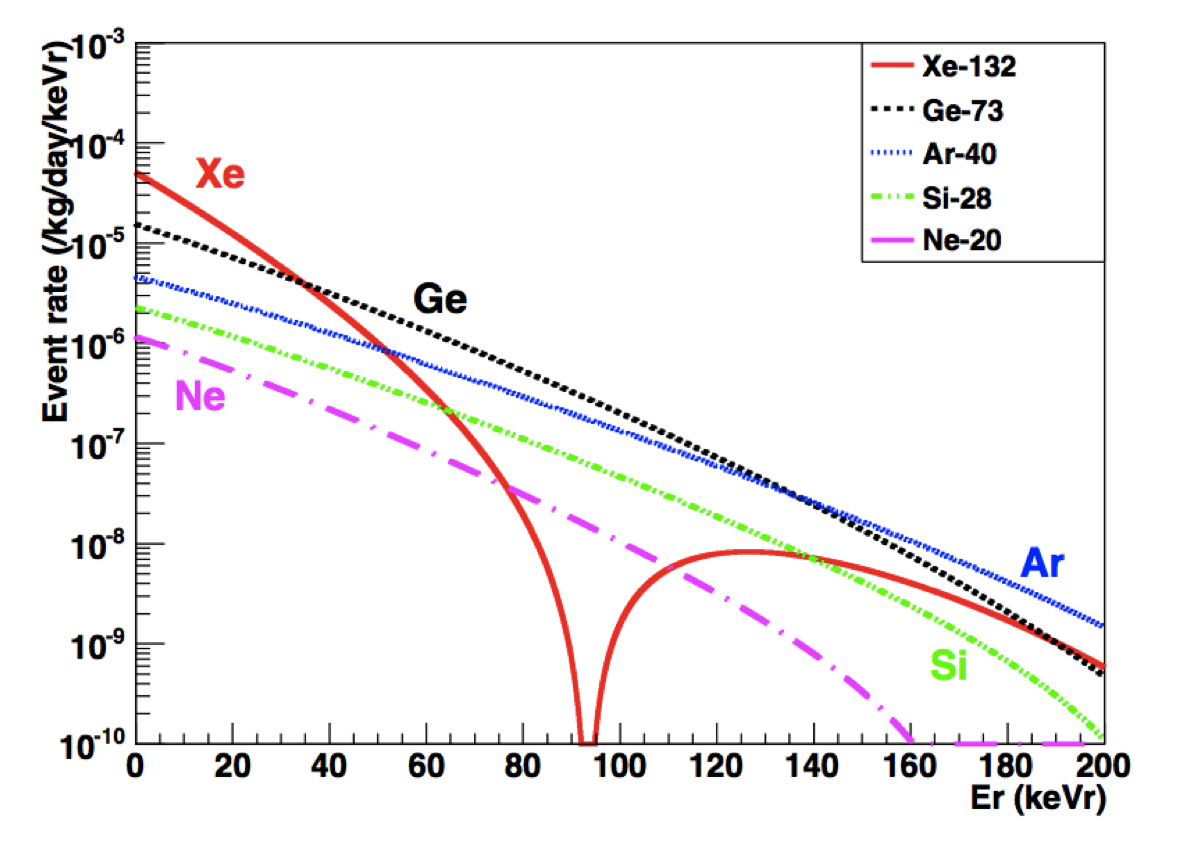
\includegraphics[width=140mm]{Intro/Ch1_Figures/Target_Nuclei.png}
\caption{Plot of WIMP event rate per kg/day/keV vs. Nuclear recoil energy (keV) for several target nuclei, using parameters from \cite{Lewin_Smith}. At low detection threshold xenon is the most attractive target nuclei. The drop off in the xenon spectral shape is due to decoherence described by the Helm factor \cite{Helm_Factor}. }
\label{fig:WIMP_Target_Nuclei}
\end{figure}


Xenon being a relatively heavy element, A=131, makes it an ideal candidate for a WIMP dark-matter search at low energy thresholds. Xenon detectors today have achieved thresholds as low as 3 $\rm keV_{nr}$ \cite{LUX_PRL}. Other common detection mediums are germanium, which is rather expensive on the ton scale, and argon which is inexpensive but contains a troublesome radioactive isotope $\rm^{39}Ar$. To probe dark matter cross sections the next generation experiments must be bigger and contain less radioactive background contamination. With current limits on the WIMP cross section a ton scale xenon experiment may only detect a handful of events per year.



\subsection{WIMP Detection Experiments}

Several experiments are currently conducting WIMP dark matter searches using several target nuclei. We have found that the interaction rate for WIMPs with target nuclei is expected to be rare. In the event that a WIMP does strike a target in the detector it will primarily interact with the nucleus, deposit energy, and traverse throughout the detector without a second interaction. Neutrons could also interact with atomic nuclei and fake a WIMP signal, however after the initial energy deposit they are likely to interact again. Thus, neutrons can be rejected by cutting multiple scatters in detectors on the scale of the neutron mean free path at an energy required to fake a WIMP signal (order 10 cm). The most common source of backgrounds are electromagnetic in nature, gammas and betas from the rock surrounding the experiment, detector components, and internal to the xenon. Just like for the case of neutrons the likelihood of a single scatter within the detector is highly unlikely. Naked beta decays are the most troublesome, appearing as a single energy deposit in the detector medium. Fortunately, electronic recoil events can be discriminated from WIMP like nuclear recoil events by more than 1/100 using the ratio of charge to light or charge to phonons produced in the interaction. Xenon based experiments currently having the best limits on WIMP nucleon cross sections \cite{LUX_PRL}.

\begin{itemize}

\item Xenon experiments: LUX \cite{LUX_PRL}, Xenon100 \cite{Xenon100} , PandaX \cite{PandaX}, XMass \cite{XMass}.

\item Argon experiments: Dark Side \cite{DarkSide}, MiniClean \cite{MiniCLEAN}. 

\item Germanium experiments: CDMS \cite{CDMS},  CoGeNT \cite{CoGeNT}.

\item Bubble chamber using fluorine: PICASSO \cite{PICASSO} (19F), COUPP \cite{COUPP} ($\rm CF_3I$).

\end{itemize}

%show WIMP limit improvement over the last 30 years


\begin{comment}
\subsection{Background Rejection}

We have found that the interaction rate for WIMPs with target nuclei is expected to be rare. In the event that a WIMP does strike a target in the detector it will primarily interact with the nucleus, deposit energy, and traverse throughout the detector without a second interaction. Neutrons could also interact with atomic nuclei and fake a WIMP signal, however after the initial energy deposit they are likely to interact again. Thus, neutrons can be rejected by cutting multiple scatters in detectors on the scale of the neutron mean free path at an energy required to fake a WIMP signal (order 10 cm). 

The most common source of backgrounds are electromagnetic in nature, gammas and betas from the rock surrounding the experiment, detector components, and internal to the xenon. Just like for the case of neutrons the likelihood of a single scatter within the detector is highly unlikely. The most troublesome of background being naked beta decays which look like a single energy deposit in the detector medium. Nuclear recoil events and electronic recoil events can be discriminated further by more than 1/100 using the ratio of charge to light or charge to phonons produced in the interaction.
\end{comment}

%% Useful LATEX tips below:
`
\begin{comment}

\section{Theorems}

\newtheorem{theorem}{Theorem}[chapter]
\begin{theorem}
This is my first theorem.
\end{theorem}


\section{Axioms}
\newtheorem{axiom}{Axiom}[chapter]
\begin{axiom}
This is my first axiom.
\end{axiom}




\begin{axiom}

This is my second axiom in chapter 1.
\end{axiom}

\section{Tables}

This is my table. 

\renewcommand{\baselinestretch}{1}
\small\normalsize

\begin{table}[h]
\caption[Short title]{Overview of test cases used in this study.}
\begin{center}
\begin{tabular}{|c|c|c|c|}
\hline
Test & Quality & Setpoint & Manipulated \\
case & variable (QV) & for QV & variables (MVs)\\
\hline \hline
TE & G/H ratio & 1.226 & D-feed SP and Reactor Level SP\\
AZ & xB($H_2O$) & & Reflux flow and $5^{th}$ Tray temperature SP\\  
\hline
\end{tabular}
\end{center}
\label{test_over}
\end{table}

\renewcommand{\baselinestretch}{2}
\small\normalsize

My table is shown above.   Normally it is double-spaced but I have inserted a command (marked in blue) to make it single-spaced and then inserted a command (again in blue) to change the text back to double-spacing.


\

\subsection{Adding Extra Space between Text and Horizontal Lines}

\renewcommand{\baselinestretch}{1}
\small\normalsize



\begin{table}[h]
\caption{Table with Extra Space between the Text and Horizontal Lines.}
\begin{center}
\begin{tabular}{|p{.5in}|p{1in}|c|p{2.25in}|}
\hline
Test case& Quality variable QV)& Setpoint for QV & Manipulated  variables (MVs)\\
\hline \hline
TE & G/H ratio & 1.226 & D-feed SP and Reactor Level SP\\ \hline
AZ & xB($H_2O$) & & Reflux flow and $5^{th}$ Tray temperature SP \\
\hline
\end{tabular}
\end{center}
\label{test_over}
\end{table}

\renewcommand{\baselinestretch}{2}
\small\normalsize

The line \begin{verbatim}\usepackage{tabls}\end{verbatim} must be inserted in the preamble of your document.
The table is set up to be single-spaced by \begin{verbatim} \renewcommand{\baselinestretch}{1} \small\normalsize\end{verbatim} before \begin{verbatim}\begin{table}\end{verbatim}.  I set the first, second, and fourth columns as paragraphs, .5in, 1in, and 2.25in wide, respectively.  I then adjusted the separation between the words and the horizontal lines to 5ex by also adding \begin{verbatim}\setlength{\tablinesep}{5ex}\end{verbatim} before the \begin{verbatim}\begin{table}\end{verbatim} command.

After typing the table I change the document to be double-spaced from this point on.


\newpage


\subsection{Numbering Figures}

If you wish your figures to be numbered 1-100 without any reference to the chapter (e.g., Figure 1.1, 2.1, etc.), change the first line of your mainthesis.tex file to read \begin{verbatim}"\documentclass[12pt]{thesis-2}".\end{verbatim}  

\subsubsection{This is a Subsubsection}

This is my first subsubsection in Chapter 1.


\section[Short Titles]{Short Titles in the Table of Contents, List of Figures, or List of Tables}

The Table of Contents, List of Figures, or List of Tables usually show the entire title of a section, subsection, etc. or table, or the entire caption of a figure.  If you put a short title in square brackets after \begin{verbatim} \section, \table, or \figure, \end{verbatim} the short title will show in your Table of Contents or lists.

\renewcommand{\baselinestretch}{1}
\small\normalsize

\begin{verbatim}
\section[Short Title]{Title of Section} 
\subsection[Short Title]{Title of Subsection} 
\end{verbatim}

or when using a caption in a figure or table
\begin{verbatim}
\caption[Short Caption]{Full text of the caption.}
\end{verbatim}

\renewcommand{\baselinestretch}{2}
\small\normalsize



\section{LaTeX -- A Typesetting Program}

A 13-page explanation of some of the features of LaTeX can be downloaded from http://www.jgsee.kmutt.ac.th/exell/General/LaTeX.html.


\section{Using Bibtex}

Using Bibtex with Latex documents is not difficult.  The bulk of the work is organizing your bibtex file, which is a data base compiled by you of the articles, books, etc. which you use in the bibliographies or reference sections of your publications.  

I have linked several files to this webpage, which will be helpful when you are using Bibtex.  These files can be downloaded from http://www.ireap.umd.edu/ireap/theses/bibtex.  Please read the file "BibtexInstructions.pdf".  The first two pages explain how to set up and run Bibtex; the remaining pages were taken from a published article and show how the references were cited in the .tex file.   The files BibtexInstructions.tex, Galactic.bib, Dottie.bib are the original .tex files used for BibtexInstructions.pdf.  The file BibtexSamples.tex contains examples of the information needed for the various publications you wish to reference (e.g., articles in refereed journals, books, unpublished articles, conference proceedings, etc.).

If you have questions concerning Bibtex, please contact me at 301-405-4955 or dbrosius at umd.edu.


\section{APS Physical Review Style and Notation Guide}

The following style guide may be downloaded from The American Physical Society at http://forms.aps.org/author/styleguide.pdf:  Physical Review Style and Notation Guide, published by The American Physical Society, compiled and edited by Anne Waldron, Peggy Judd, and Valerie Miller, February 1993.  It may be old, but it is very useful.
 
 \end{comment}
